{$\space$\par}
\vspace{0.5cm}
\justifying
\section*{{\bfseries \LARGE Questão 5 -} {\bfseries \large  Estime os parâmetros das leis de potência que descrevem: 
\begin{enumerate}
    \item a distribuição de massas das estrelas primárias (M1);
    \item  a distribuição de massa das estrelas secundárias (M2). Represente ambas as distribuições empíricas em um gráfico quantil-quantil.
\end{enumerate}}}

\vspace{0.8cm}

\textcolor{red}{A distribuição de Pareto é muito utilizada em astronomia devido às diferentes escalas envolvidas na área. Nessa amostra de dados, temos a massa das estrelas de vários sistemas binários em logaritmo. Para estimar os parâmetros dessas leis de potência, vou utilizar o método de mínimos quadrados:}

\vspace{0.8cm}

\begin{lstlisting}
    binaries = read.table('/content/belikov.dat', header=T, sep='|')

    pareto.MLE = function(X) {
      n = length(X)
      m = min(X)
      a = n/sum(log(X)-log(m)) 
      return(c(m,a))
      
    # Fitting
    params_m1 = pareto.MLE(10**binaries$M1)
    params_m2 = pareto.MLE(10**binaries$M2)
    cat('Fit for primary stars (location, shape):',params_m1[1],params_m1[2],'\n')
    cat('Fit for secundary stars (location, shape):',params_m2[1],params_m2[2])

    # Creating theoretical values from fitted distribution
    fit_m1 = log10(rpareto(length(binaries$M1), shape=params_m1[2], scale=params_m1[1]))
    fit_m2 = log10(rpareto(length(binaries$M2), shape=params_m2[2], scale=params_m2[1]))

    # QQ plot for Primaries
    qqplot(binaries$M1, fit_m1, xlab = "Primary mass (log)", ylab = "Primary mass from fit (log)")
    lines(binaries$M1, binaries$M1, col='red', lwd=4)
    legend('topleft', legend='Q_empirical = Q_fitted', lwd=4, col='red', box.lwd=0)

    # QQ plot for secundaries
    qqplot(binaries$M2, fit_m2, xlab = "Secundary mass (log)", ylab = "Secundary mass from fit (log)")
    lines(binaries$M2, binaries$M2, col='red', lwd=4)
    legend('topleft', legend='Q_empirical = Q_fitted', lwd=4, col='red', box.lwd=0)
}
\end{lstlisting}

\begin{lstlisting}
    Fit for primary stars (location, shape): 1.16681 0.1031938 
    Fit for secundary stars (location, shape): 1.135011 0.1446229
\end{lstlisting}

\begin{figure}
    \centering
    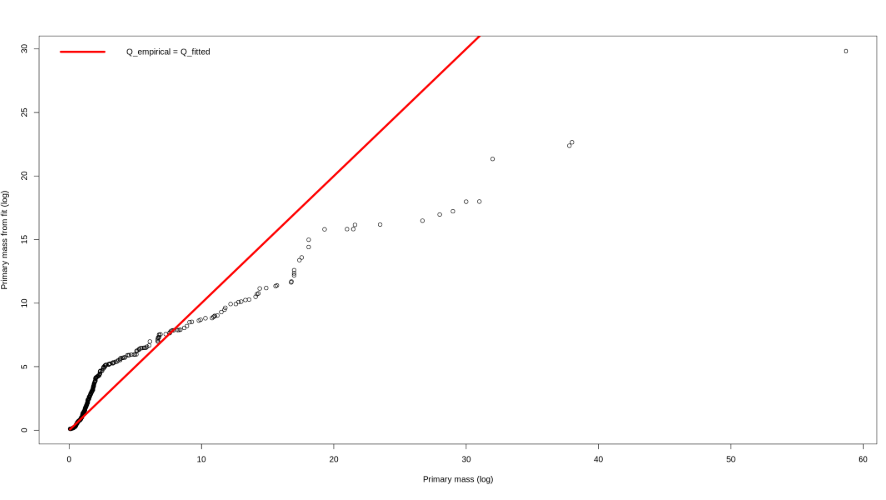
\includegraphics[width=0.9\linewidth]{Figuras/Captura de tela 2025-06-01 113313.png}
    \caption{QQ plot com a massa primaria no eixo x e Pareto ajustada no eixo y. A linha vermelha representa o caso onde os quantis dos dados e da distribuição ajustada são iguais.}
\end{figure}

\begin{figure}
    \centering
    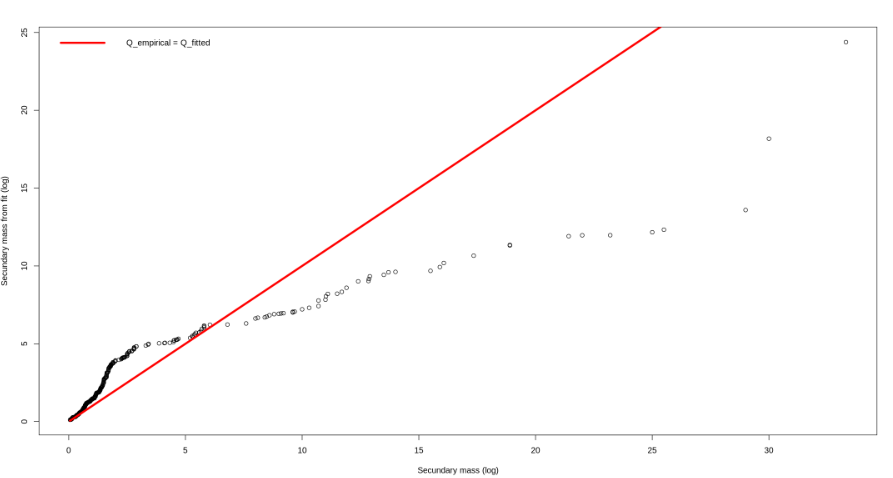
\includegraphics[width=0.9\linewidth]{Figuras/Captura de tela 2025-06-01 113326.png}
    \caption{QQ plot com a massa secundária no eixo x e Pareto ajustada no eixo y. A linha vermelha representa o caso onde os quantis dos dados e da distribuição ajustada são iguais.}
\end{figure}